\section{Optimisations}
\label{sec:optimisations}
Due to the relatively poor scaling performance and the identification of the current most significant bottlenecks, optimisations are being applied to the QNLP library for the final scaling experiments to be carried out during the last stage of the project. These optimisations mainly consist of algorithmic changes to the decomposition of the $n$-controlled unitary (\textit{NCU}) operations into the fundamental gate-set made available by the underlying quantum simulator. Following the gate-set decomposition procedures discussed in \cite{Barenco_1995}, we can achieve an order or magnitude reduction in gate operations. The scaling of the decomposition for both the default and optimised routines is given by Fig.~\ref{fig:ncu_opt}.


\begin{figure}[!h]
\centering
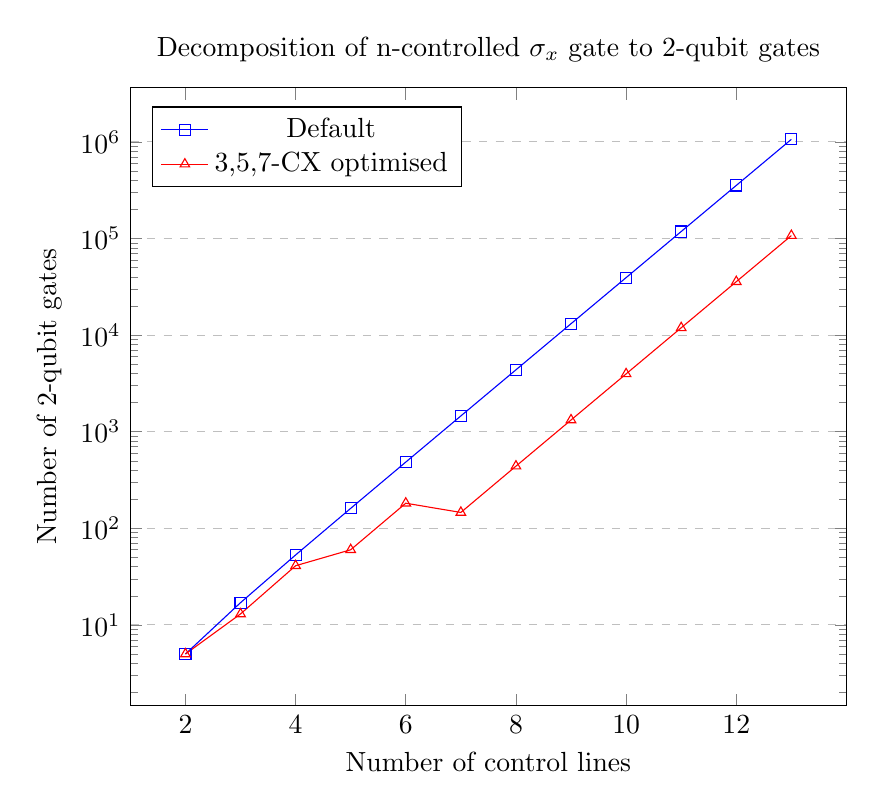
\begin{tikzpicture}
\begin{axis}[
    title={Decomposition of n-controlled $\sigma_x$ gate to 2-qubit gates},
    xlabel={Number of control lines},
    ylabel={Number of 2-qubit gates},
    xmin=1, xmax=14,
    %ymin=0, ymax=1200,
    xtick={2,4,6,8,10,12},
    ytick={1,10,100, 1000, 10000, 100000,1000000},
    legend pos=north west,
    ymajorgrids=true,
    grid style=dashed,
    ymode=log,
    scale only axis,
    width=0.75\textwidth,
]
\addplot[
    color=blue,
    mark=square,
    ]
    coordinates {
    (2, 5)
    (3, 17)
 (4, 53)
 (5, 161)
 (6, 485)
 (7, 1457)
 (8, 4373)
 (9, 13121)
 (10, 39365)
 (11, 118097)
 (12, 354293)
 (13, 1062881)
    };
\addplot[
    color=red,
    mark=triangle,
    ]
    coordinates {
    (2,5)
(3, 13)
 (4, 41)
 (5, 60)
 (6, 182)
 (7, 146)
 (8, 440)
 (9, 1322)
 (10, 3968)
 (11, 11906)
 (12, 35720)
 (13, 107162)
 };
    \legend{Default, {3,5,7}-CX optimised} 
\end{axis}
\end{tikzpicture}
\caption{The 2-qubit gate operations generated by the n-controlled unitary decomposition. The default method is the current implementation, where the optimised {3,5,7}-method optimises the decompositions where applicable.}
\label{fig:ncu_opt}
\end{figure}

While using the 3,5,7 optimisations still scales exponentially, the offset for larger control operations shows approximately an order of magnitude improvement in number of calls. This will be essential to attempting large-scale runs of the end-to-end implementation during the final stage of the project.
